% Copyright 2004 by Till Tantau <tantau@users.sourceforge.net>.
%
% In principle, this file can be redistributed and/or modified under
% the terms of the GNU Public License, version 2.
%
% However, this file is supposed to be a template to be modified
% for your own needs. For this reason, if you use this file as a
% template and not specifically distribute it as part of a another
% package/program, I grant the extra permission to freely copy and
% modify this file as you see fit and even to delete this copyright
% notice. 

\documentclass{beamer}

% There are many different themes available for Beamer. A comprehensive
% list with examples is given here:
% http://deic.uab.es/~iblanes/beamer_gallery/index_by_theme.html
% You can uncomment the themes below if you would like to use a different
% one:
%\usetheme{AnnArbor}
%\usetheme{Antibes}
%\usetheme{Bergen}
%\usetheme{Berkeley}
%\usetheme{Berlin}
%\usetheme{Boadilla}
%\usetheme{boxes}
%\usetheme{CambridgeUS}
%\usetheme{Copenhagen}
%\usetheme{Darmstadt}
%\usetheme{default}
%\usetheme{Frankfurt}
%\usetheme{Goettingen}
%\usetheme{Hannover}
%\usetheme{Ilmenau}
%\usetheme{JuanLesPins}
%\usetheme{Luebeck}
\usetheme{Madrid}
%\usetheme{Malmoe}
%\usetheme{Marburg}
%\usetheme{Montpellier}
%\usetheme{PaloAlto}
%\usetheme{Pittsburgh}
%\usetheme{Rochester}
%\usetheme{Singapore}
%\usetheme{Szeged}
%\usetheme{Warsaw}


% Customize Warsaw color 
\setbeamercolor*{palette primary}{use=structure,fg=white,bg=red!50!black}
\setbeamercolor*{palette secondary}{use=structure,fg=white,bg=red!60!black}
\setbeamercolor*{palette tertiary}{use=structure,fg=white,bg=red!70!black}

% Customize Warsaw block title and background colors
\setbeamercolor{block title}{bg=red!50!black,fg=white}


% List your packages here

\usepackage[colorinlistoftodos]{todonotes}
\usepackage{graphicx}
\usepackage{fancyvrb}

\title[Progress Update]{A Generalized Open Source Platform for Building Energy Management}

% % A subtitle is optional and this may be deleted
% \subtitle{Product Proposal}

\author[B.~Lauer]{Brian~Lauer \\\and
Advisor: Dr. Suruz Miah}
% - Give the names in the same order as the appear in the paper.
% - Use the \inst{?} command only if the authors have different
%   affiliation.

\institute[Bradley University] % (optional, but mostly needed)
{
  Department of Electrical and Computer Engineering\\
  Bradley University\\
  1501 W. Bradley Avenue\\
  Peoria, IL, 61625, USA
}
% - Use the \inst command only if there are several affiliations.
% - Keep it simple, no one is interested in your street address.

\date[April~3,~2020]{Friday, April~3,~2020}
% - Either use conference name or its abbreviation.
% - Not really informative to the audience, more for people (including
%   yourself) who are reading the slides online

\logo{\hfill\href{http://www.bradley.edu}{
\includegraphics[width=0.75cm]{../figs/logoBU1-Print}}}  % place logo in every page 

% This is only inserted into the PDF information catalog. Can be left
% out. 

% If you have a file called "university-logo-filename.xxx", where xxx
% is a graphic format that can be processed by latex or pdflatex,
% resp., then you can add a logo as follows:

% \pgfdeclareimage[height=0.5cm]{university-logo}{university-logo-filename}
% \logo{\pgfuseimage{university-logo}}


% Let's get started
\begin{document}

\begin{frame}
  \titlepage
\end{frame}

\begin{frame}{Outline}
  \tableofcontents
  % You might wish to add the option [pausesections]
\end{frame}

% Section and subsections will appear in the presentation overview
% and table of contents.
\section{Objectives}

\begin{frame}{Objectives}{}
  % applications of mobile robot navigation and problem description
  \begin{itemize}
	\item Write networking code for communicating with the DC motor and WeMo switch
	\item Build simple login page  
  \end{itemize}
\end{frame}

%----------------------------------
\section{ESP8266 MCU Board}

\begin{frame}{ESP8266}{}
\begin{itemize}
\item Made the decision to control DC motor with only a ESP8266 Node MCU board
\item Plan to swap out Raspberry Pi and XBee module
\begin{figure}
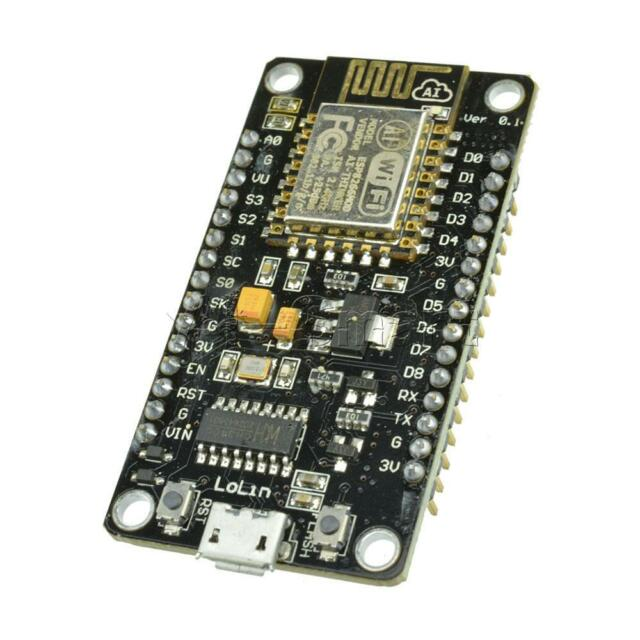
\includegraphics[scale=0.89]{../figs/img/esp8266NodeMCU}
\caption{ESP8266 Node MCU Lua V3 courtesy of ebay.com}
\end{figure}
\end{itemize}
\end{frame}

\section{ESP8266 MCU Board}
\begin{frame}{ESP8266 MCU Board}{}
\begin{itemize}
\item Wrote a primitive Python TCP/IP web server to run on the board
\item File must be named \texttt{main.py} to allow execution on start up
\item Continually accepts connections from clients connected to the same network (\texttt{server\_socket.accept()})
\item Continually accept commands from remote clients (\texttt{client\_socket.recv(BUFFER\_SIZE)})
\item 'ON' toggles a GPIO pin on while 'OFF' toggles the GPIO pin off
\item PWM value can be set on a separate pin using the format \texttt{'PWM: value'} where \texttt{value} is an integer
\item Could be useful in controlling the speed of the motor
\end{itemize}
\end{frame}

\section{WeMo Switch Discovery and Control}
\subsection{Explanation of Discovery}
\begin{frame}{WeMo Switch Discovery and Control}{Explanation of Discovery}
\begin{itemize}
\item Gained a better understanding of the code in the BEMOSS repository for controlling the WeMo switch
\item SSDP (Simple Service Discovery Protocol) utilized for discovery of the switch and other UPNP (Universal Plug and Play) devices
\item UDP socket is created and a HTTP request is sent over UDP to address "239.255.255.250", 1900
\item HTTP method: 'M-SEARCH', url: '*', version: HTTP/1.1
\begin{figure}
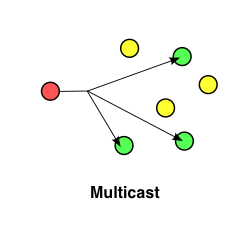
\includegraphics[scale=0.3]{../figs/img/multicast_routing_diagram}
\caption{Courtesy of https://williamboles.me/discovering-whats-out-there-with-ssdp/}
\end{figure}
\end{itemize}
\end{frame}

\section{WeMo Switch Control}
\begin{frame}{WeMo Switch Discovery and Control}{Explanation of Discovery}
\begin{itemize}
\item Headers of multicast http request include
\item \texttt{HOST} - where the message will be sent ("239.255.255.250", 1900)
\item \texttt{MAN} - message type which is always \texttt{ssdp:discover}
\item \texttt{ST} - search type, in the case of WeMo switch is "upnp:rootdevice"
\item \texttt{MX} - time (seconds) a root device can take before responding
\end{itemize}
\begin{figure}
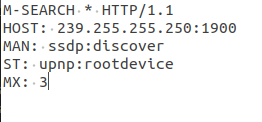
\includegraphics[scale=0.5]{../figs/img/upnpRequest}
\caption{Request used in WeMo API in BEMOSS}
\end{figure}
\end{frame}

\subsubsection{Explanation of Control}
\begin{frame}{WeMo Switch Discovery and Control}{Explanation of Control}
\begin{itemize}
\item Responses returned by available UPNP devices contain a header \texttt{location} which specifies location of the XML file listing services available and metadata
\item WeMo switch contains file called \texttt{setup.xml}
\item XML file is requested and parsed in Python using \texttt{xml.dom.minidom} module
\item Tags like \texttt{modelName}, \texttt{manufacturer}, \texttt{serialNumber} and \texttt{deviceType} can be used for further identifying the device
\end{itemize}
\end{frame}

\begin{frame}{WeMo Switch Discovery and Control}{Explanation of Control}
\begin{itemize}
\item Once address of device is found request can be made
\item Body must be created with binary state and or brightness depending on model of switch
\end{itemize}
\begin{figure}
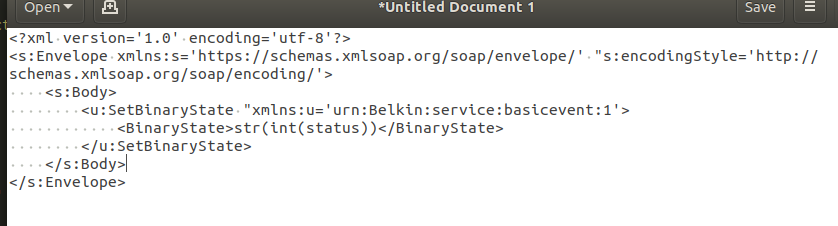
\includegraphics[scale=0.3]{../figs/img/soapRequestWeMO}
\caption{Body of request}
\end{figure}
\end{frame}

\section{Front End Work}
\begin{frame}{Front End Work}{}
\begin{figure}
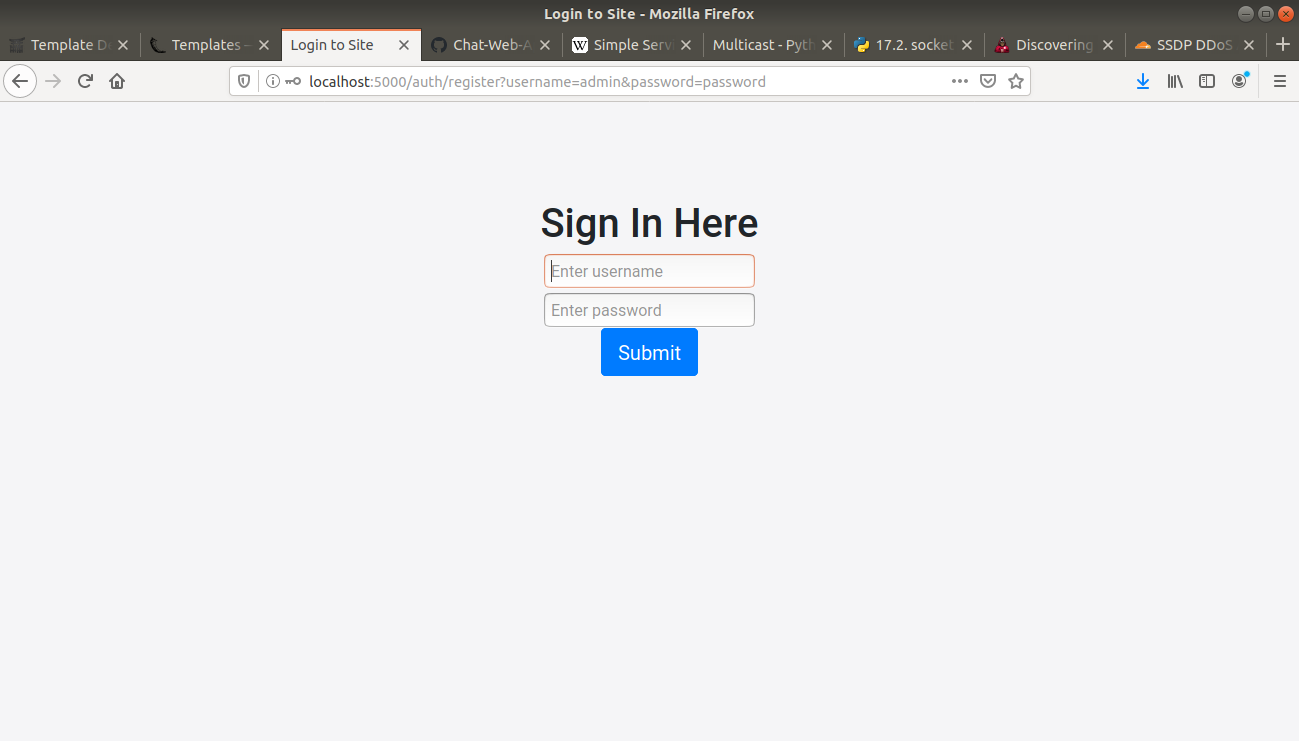
\includegraphics[scale=0.25]{../figs/img/signInPage}
\caption{Prototype login page for BEMS}
\end{figure}
\end{frame}

\section{Front End Work}
\begin{frame}{Front End Work}{}
\begin{figure}
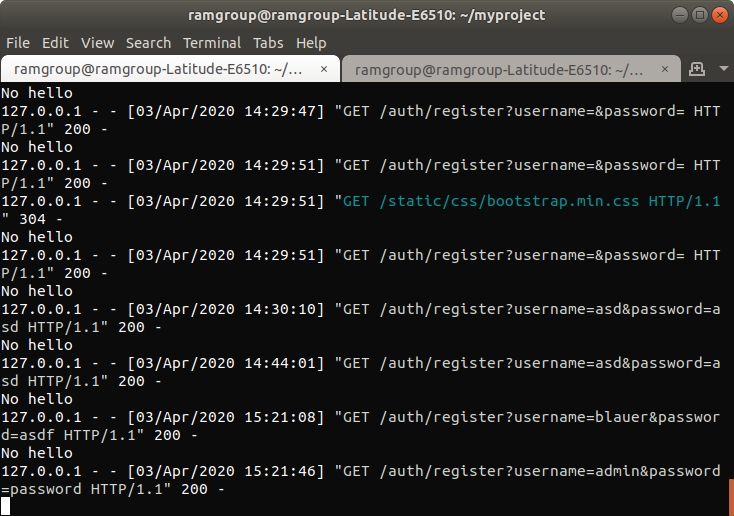
\includegraphics[scale=0.35]{../figs/img/noPost}
\caption{Flask debug console capture}
\end{figure}
\end{frame}

\section{Objectives for Coming Weeks}
\begin{frame}{Objectives for Coming Weeks}{}
\begin{itemize}
\item Create plan for software development
\item Setup SQLite database for users and devices
\item Fix problem with login page
\item Read papers on agent based architecture
\end{itemize}
\end{frame}

\begin{frame}
\center
\Huge
Any Questions?
\end{frame}
\end{document}



%%% Local Variables:
%%% mode: latex
%%% TeX-master: t
%%% End:
